\documentclass{../../text-style}

\texttitle{Контейнеры и генерики}

\begin{document}

\maketitle
\thispagestyle{empty}

\section{Контейнеры}

Редко встречаются программы, которые используют определенное, заранее строго заданное число объектов с известным временем жизни. В общем случае (а особенно в случае event-driven приложений) объекты в программах создаются, используются и удаляются в зависимости от реализуемых алгоритмов, что может потребовать создания произвольного количества объектов в любой момент времени. Практически все языки предоставляют те или иные способы для организации работы с <<похожими объектами>>. Одними из таких конструкций в C\# являются массивы. В C/C++ тоже были массивы, в C\# массив --- это объект с некоторыми полезными полями, но суть это мало меняет: массивы хороши, когда число элементов фиксировано и когда критично время доступа к ним (хотя если кто-то осознал, что ему стало критично время исполнения программы, то ему, видимо, стоит подумать об использовании более подходящего языка программирования). Хранить же переменное (и, что важно, заранее неизвестное) число значений в массиве ужасно неудобно --- придётся каждый раз, когда значения перестают помещаться в массив, выделять новый кусок памяти под весь массив, и копировать старые значения туда.

Собственно, чтобы можно было хранить данные, не заботясь о выделении памяти, размерах массивов и всём таком, и существуют контейнеры (они же коллекции) библиотеки .NET. Коллекции реализуют разные абстрактные типы данных, начиная от простых списков на массивах (или на указателях), заканчивая всякими словарями на самобалансирующихся деревьях. Контейнеры в .NET бывают генериковыми и негенериковыми. О том, что такое генерики (а также о том, что такое на самом деле генерики) будет чуть попозже, начнём с негенериковых коллекций.

\section{Негенериковые коллекции}

Негенериковые коллекции описаны в основном в неймспейсе System.Collections (ещё немного --- в System.Collections.Specialized). На самом деле негенериковыми коллекциями пользуются нынче очень редко, они остались с тех давних времён, когда .NET ещё не поддерживал генерики. Тем не менее, негенериковые коллекции концептуально устроены так же, как генериковые, и их полезно рассмотреть сначала, чтобы не отвлекаться на незнакомый синтаксис. Самые интересные коллекции из System.Collections такие:

\begin{itemize}
    \item ArrayList --- список на массивах. Сам берёт на себя работу по изменению размера, обращение к элементу по индексу работает за константное время, но добавление элемента может привести к копированию массива, что потребует линейного времени (а может и не привести, потому что он меняет свой размер обычно степенями двойки). Реализует интерфейсы IList, ICollection, IEnumerable, ICloneable.
    \item BitArray --- примерно то же самое, что и список, только для булевых значений, эффективно использует память. Реализует ICollection, IEnumerable, ICloneable.
    \item Hashtable --- словарь, хранящий пары <<ключ-значение>>, и позволяющий за константное время получать значение по ключу. Реализует IDictionary, ICollection, IEnumerable, ICloneable.
    \item Queue --- очередь. Реализует ICollection, IEnumerable, ICloneable.
    \item SortedList --- словарь из пар <<ключ-значение>>, медленнее, чем Hashtable, зато позволяющий обращаться к элементам по индексу. Реализует интерфейсы IDictionary, ICollection, IEnumerable, ICloneable.
    \item Stack --- внезапно, стек. Реализует ICollection, IEnumerable, ICloneable.
\end{itemize}

Обратите внимание, что каждая коллекция реализует пачку интерфейсов, причём я специально обращаю на это внимание. Во-первых, интерфейсы дают несколько больший уровень общности и сокрытия деталей реализации, так что если вы напишете код, которому нужно только ходить по коллекции (что обеспечивает интерфейс IEnumerable), он будет работать для вообще всех коллекций, от стека до хеш-таблицы. Во-вторых, интерфейсы очень многое говорят о функциональности, которую коллекции реализуют. Основные интерфейсы, используемые в дотнетовских коллекциях, таковы.

\begin{center}
    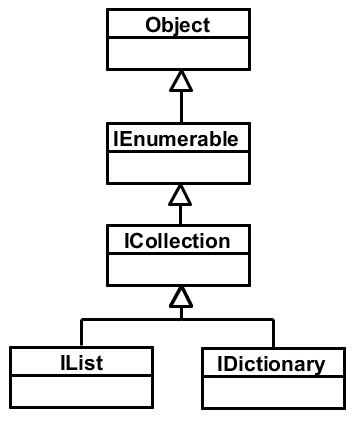
\includegraphics[width=0.4\textwidth]{interfaces.png}
\end{center}

\begin{itemize}
    \item ICollection --- абстракция <<коллекции>>, которая знает свой размер, куда можно добавлять/удалять элементы, проверять принадлежность элемента коллекции, очищать коллекцию.
    \item ICloneable --- абстракция <<штуки, которую можно копировать>>. Декларирует единственный метод Clone, который должен быть реализован как возвращающий глубокую копию объекта. Для тех, кто не в курсе, глубокая (deep) копия --- это когда копируется сам объект, объекты, на которые он ссылается, объекты, на которые ссылаются объекты, на которые он ссылается и т.д., мелкая (shallow) копия --- когда копируется только сам объект, ссылки в объекте-копии указывают на те же объекты, на которые они указывали в объекте-оригинале.
    \item IDictionary --- словарь, коллекция пар <<ключ-значение>>. В дополнение к методам интерфейса ICollection, который он реализует, содержит методы поиска значения по ключу, удаления по ключу, получения списка ключей и списка значений, и подобные.
    \item IEnumerable --- абстракция <<штуки, из которой можно последовательно получать элементы>>. Декларирует только один метод --- получение энумератора.
    \item IEnumerator --- абстракция курсора, позиции, или чего-то такого, что позволяет ходить по коллекции. Дотнетовская реализация паттерна <<Итератор>>. Про то, что такое паттерны, будет подробно в следующем семестре, на пальцах итератор --- это класс, инкапсулирующий в себе правило обхода коллекции. Вот в прошлом семестре мы писали, например, списки, которые сами содержали методы, позволявшие по ним ходить (next, например), принимавшие позицию. Так можно, но вообще, хранение элементов и обход элементов --- это разные задачи, поэтому согласно принципам ООП, должны быть разделены по разным классам. В конце концов, вариантов обхода может быть много: для списка, например, с начала или с конца, для дерева --- preorder, postorder и inorder. Простое и общепринятое решение этой проблемы --- реализовать алгоритм в отдельном классе, объекты которого могла бы создавать сама коллекция, предоставить этому классу эксклюзивный доступ к внутренней структуре коллекции (в C++ это можно делать с помощью ключевого слова friend, в Java --- с помощью того, что вложенные классы хранят ссылку и имеют доступ к полям объемлющего класса, в C\# придётся ссылку на объемлющий класс хранить явно, но доступ к private-полям у вложенного класса всё равно есть). Потом объект этого класса можно использовать уже в отрыве от самой коллекции, можно насоздавать хоть сотню энумераторов и использовать их для того, чтобы ходить по коллекции независимо. Энумератор имеет всего три метода --- Current (на самом деле, это свойство), возвращающий текущий элемент, MoveNext --- перейти на следующий элемент, и Reset --- поставить энумератор на начальную позицию, которая до первого элемента в коллекции (то есть, чтобы получить первый элемент, надо сделать Reset, MoveNext и Current). Кстати, про энумераторы и IEnumerable знает компилятор, так что если коллекция (в том числе и ваша, рукописная) правильно реализует эти интерфейсы, по ней можно будет ходить циклом foreach. Например, \mintinline{csharp}|foreach (var i in list) { Console.Write(i); }|. При обходе коллекции энумератором менять её нельзя (иначе энумератор может остаться указывающим на удалённый элемент, например). Энумератор может детектить изменение коллекции и попытка вызвать MoveNext приведёт к исключению. При этом Current должен всё равно работать и возвращать последний элемент, который видел энумератор, даже если тот был удалён.
    \item IList --- представляет абстракцию коллекции, к элементам которой можно обращаться по индексу.
\end{itemize}

Теперь про то, почему негенериковыми коллекциями никто не пользуется. Первая проблема (не принципиальная) заключается в том, что негенериковые коллекции хранят все свои элементы как object-ы, так что если мы хотим положить в коллекцию value type (тип, значения которого хранятся на стеке, например, int), компилятору придётся явно отконвертировать value type в object (выполнив операцию боксинга (boxing)), а при извлечении элемента из коллекции выполнять анбоксинг (unboxing). Это небыстро. Вторая проблема (принципиальная) состоит в типобезопасности. В негенериковый контейнер можно класть объекты разных типов. То есть, список строк, в котором некоторые элементы --- целые числа. Или положить в стаканчик для карандашей линейный корабль. И система типов языка ничего не сможет с этим поделать, потому что для неё содержимое контейнера --- просто object, и вся ответственность за корректное приведение элементов к правильному типу лежит на программисте. А программисты ошибаются. Кроме того, это неудобно --- забирать из коллекции object и делать ему понижающее приведение, например, оператором as. Каждый раз. Поэтому придумали понятие <<генерик>>, дающее возможность указать, значения каких типов может хранить коллекция. Так пишут в книжках типа <<C\# для профессионалов>>, <<С\# для экспертов>> и т.д. Однако же у нас тут университет, а не трёхмесячные курсы, поэтому вам придётся узнать, что такое генерики на самом деле.

\section{Параметрический полиморфизм}

Генерик --- это функция над типами. Для этого, наверное, надо ещё раз напомнить, что такое тип и для чего они нужны. Данные в памяти хранятся просто как строки битов, и что означает каждая конкретная строка --- вопрос её интерпретации. Одна и та же последовательность бит, в зависимости от того, как её прочитать, может быть числом, строкой, или вообще кодом функции. Или, например, есть у нас теория множеств (кстати, хороший пример нетипизированной формальной системы), с её помощью можно определить понятие <<число>> (как множества с подмножествами разного уровня вложенности, например, \{ \} будет 1, \{ \{ \} \} --- 2, и т.д.), можно даже определить понятие <<сложение>>, как операцию, которая принимает представления двух чисел в виде множеств, и возвращает  представление в виде множества суммы этих чисел. Проблемы начинаются, когда мы этой функции передадим не число. Что тогда будет, вообще говоря, не определено, что, наверное, не очень хорошо для компьютерной программы. И вообще, любое осмысленное множество значений всегда естественным образом распадается на подмножества, которые используются более-менее одинаковым образом --- зачатки типов. Однако сломать такую <<систему типов>> очень просто --- что будет теоретико-множественным объединением операции <<сложение>> и числа 1?

Для того, чтобы таких вопросов не возникало, вводятся формальные системы типов, которые просто запрещают ситуации, в которых такие вопросы могут возникнуть. Кстати, с теорией множеств без системы типов случается печаль, которая называется парадоксом Рассела: <<Пусть А --- множество всех множеств, которые не содержат себя в качестве своего элемента. Содержит ли А само себя в качестве элемента? Если предположить, что содержит, то мы получаем противоречие с <<не содержат себя в качестве своего элемента>>. Если предположить, что  не содержит себя, как элемент, то вновь возникает противоречие, ведь А — множество всех множеств, а значит, должно содержать все возможные элементы, включая и себя>>. Собственно, систему типов можно рассматривать как <<одежду>> для нетипизированного внутреннего представления значений. Объекты какого-либо типа допускают только операции, которые можно совершать над объектами этого типа, причём зачастую имеют внутреннее представление, упрощающее совершение этих операций (поэтому, кстати, арабские цифры победили римские). Пока ограничения, накладываемые системой типов, выполняются, во внутреннее представление нельзя <<влезть>> и всё испортить (например, не получится вызвать благодаря парадоксу Рассела массовой депрессии у математиков начала 20-го века).

Вернёмся ближе к программированию. В языках программирования используются довольно сложные системы типов и средства автоматической проверки программы на соответствие этим системам. Языки программирования бывают:

\begin{itemize}
    \item со статической типизацией --- когда тип любой переменной и любого выражения точно известен во время компиляции. Это хорошо, поскольку гарантирует отсутствие ошибок, связанных с типами, но зачастую накладывает слишком жёсткие ограничения.
    \item с сильной типизацией --- более мягкое требование, что корректность всех выражений с точки зрения системы типов может быть проверена во время компляции, хотя конкретные типы конкретных частей выражения могут быть неизвестны. Любой язык со статической типизацией является языком с сильной типизацией, но не наоборот. В современной литературе и статическую, и сильную типизацию отождествляют.
\end{itemize}

Собственно, генерики свойство статической типизации могут нарушать, тем не менее, всегда можно доказать корректность с точки зрения типов операций, которые осуществляются в генериках, то есть системы типов с генериками остаются сильно типизированными, хотя и не статически типизированными.

Теперь, собственно, про полиморфизм. Тип можно рассматривать как набор значений, то есть как подмножество множества всех допустимых значений. Подмножества могут перекрываться, так что теоретически ничто не мешает одному значению принадлежать сразу нескольким типам (самое забавное, что на практике очень часто используется одно значение, принадлежащее бесконечному множеству типов --- null). Бывают системы типов, где любая переменная или функция имеет ровно один тип, такие системы типов называются мономорфными. Полиморфные системы типов --- системы типов, в которых одна переменная может иметь несколько типов сразу. Полиморфные типы --- это типы, операции которых могут быть применены к операндам более чем одного типа.

Полиморфизма можно добиться по-разному. Выделяют две крупные группы полиморфизма --- универсальный полиморфизм и ad-hoc полиморфизм. Универсальный полиморфизм в свою очередь разделяется на параметрический полиморфизм и полиморфизм подтипов, ad-hoc полиморфизм --- на перегрузку и приведение. Собственно, ad-hoc полиморфизм прост и понятен, простой пример взаимосвязи видов ad-hoc полиморфизма, после которого станет ясно, о чём идёт речь: выражение <<1 + 1.0>>. Добиться компилируемости этого выражения можно разными способами: либо четыре раза перегрузив оператор <<+>> (int + int, int + float, float + int, float + float), либо два раза перегрузив оператор <<+>> (int + int, float + float) и позволив int-ам автоматически приводиться к float-ам, либо вообще не перегружая <<+>>, а просто определив его как float + float, и приводить все int-ы к float-ам всегда (а поскольку приведение требует преобразования внутреннего представления чисел, получить печаль со скоростью работы).

Полиморфизм подтипов проще всего понимать как сабтайпинг, или обычное наследование. Поскольку яблоко --- это фрукт, то все действия, применимые к фруктам, автоматически можно применить и к яблокам. Наследованием дело не ограничивается, ведь интервал [1..10] является подинтервалом интервала [1..100], так что элементы первого интервала могут быть использованы везде, где могут быть использованы элементы второго интервала, но наследование на практике используется гораздо чаще, чем такие формы полиморфизма. 

Параметрический полиморфизм предполагает у полиморфной операции наличие явных или неявных параметров-типов, которые и определяют типы аргументов для каждого применения этой операции, например, функция id: x : ‘T -> x : ‘T. Тип ‘T будет известен только там, где мы вызываем эту функцию, и может быть разным в разных ситуациях, например, можно вызвать id как id<int>(2), а можно как id<string>("fhtagn"). Функции, обладающие параметрическим полиморфизмом, называются генерик-функциями, на практике ещё активно применяют генерик-классы, которые с точки зрения теории типов можно в каком-то смысле рассматривать просто как набор генерик-функций. Простой пример генерик-класса --- список List<’T>, он может хранить в себе некоторые элементы, а какие именно это будут элементы, мы определяем в момент его использования.

Универсальный полиморфизм называется универсальным потому, что операция может быть применена к потенциально бесконечному множеству типов, в отличие от ad-hoc полиморфизма, где набор допустимых типов ограничен. Например, если операция применима к обьектам, то ей в качестве параметров можно передавать яблоки, подводные лодки, что угодно, что наследуется от обьектов. Так же и с параметрическим полиморфизмом --- функция id: x -> x может быть применена к вообще каким угодно значениям. А вот с ad-hoc полиморфизмом не так, для каких типов функция перегружена, для таких её и можно вызывать. То же самое с приведением, оно будет работать только для типов, для которых оно определено. Кроме того, в случае с перегрузкой и приведением разные <<варианты>> функции могут быть реализованы совершенно по-разному, а в случае универсального полиморфизма будет честно выполняться один и тот же код. Поэтому универсальный полиморфизм называют <<истинным>> полиморфизмом, и именно он особенно интересен с теоретической точки зрения. При этом параметрический полиморфизм наиболее выразителен, поскольку полиморфизм подтипов выражается через него.

Собственно, любой язык содержит в себе некоторое количество элементарных типов (инты, булевый тип, символы), и конструкторы типов, позволяющие из более простых типов строить более сложные (массивы, записи, классы). Можно говорить о подьязыке выражений над типами, как наборе конструкторов типов и элементарных типов, и над множеством типов определить, например, операцию равенства --- два типа равны, если их структура совпадает. Такой подход к равенству называется структурным равенством типов, в противоположность равенству по имени, когда два типа равны, если их имена совпадают. В обычных языках, типа C\#, используется именно равенство по имени, так что два одинаковых типа считаются системой типов языка разными. С точки зрения выражений над типами генерик можно рассматривать как функцию над типами --- функцию, принимающую параметры-типы и возвращающую тип конкретной специализации генерика.

Подробности про системы типов можно почитать в классической статье Cardelli, Luca, and Peter Wegner. <<On understanding types, data abstraction, and polymorphism.>> ACM Computing Surveys (CSUR) 17.4 (1985): pp. 471-523. По крайней мере, её начало может быть весьма полезным чтением. Лука Карделли, автор статьи, вроде как до сих пор работает в Microsoft Research.

\section{Генерики в .NET}

Теперь, чтобы связать теорию с практикой, рассмотрим, как это всё работает в .NET. В C\# генерики имеют параметры-типы, задаваемые в угловых скобках, например, в неймспейсе System.Collections.Generic есть класс List<T>, который можно использовать, подставляя вместо T конкретный тип: \mintinline{csharp}|List<string> listOfStrings = new List<string>();|. В такой список можно положить только строки и забрать только строки, попытка положить туда, например, целое число приведёт к ошибке компиляции. В стандартной библиотеке бывают и генерик-методы, например, Array.Sort<T>, которые можно использовать, например, вот так:

\begin{minted}{csharp}
int[] myInts = {1, 5, 2, 8, 4};
Array.Sort<int>(myInts);
\end{minted}

Генерики в .NET --- это нечто среднее между шаблонами в C++ и генериками в Java. В Java применяется подход, называемый <<стирание типа>> --- генерик существует только во время компиляции, в байт-коде это обычная коллекция из Object-ов. Это позволяет Java-машине не заморачиваться с генериками вообще, делает возможным каст от одного генерик-типа к другому, и имеет все преимущества генериков, например, типобезопасность --- компилятор-то про генерики знает. Но в Java в генерик нельзя класть элементарные типы, например, числа --- они должны быть обёрнуты в Object, что убивает производительность.

В C++ же наоборот, для каждого генерика и каждого его параметра-типа генерируется и компилируется новый код, так что для любого типа всё будет работать, и среда времени выполнения, наоборот, не знает про другие варианты генерика, для неё это обычный метод или класс, работающий с обычными типизированными данными. Это сильно расширяет возможности генериков (например, можно использовать методы у параметра-типа, не накладывая ограничения на сам параметр-тип; когда мы его подставим, компилятор проверит, что всё норм), но так очень сильно растёт размер бинарного файла.

В .NET виртуальная машина знает про генерики и параметры-типы, но генерит одну реализацию в байт-коде для всех ссылочных типов (как Java, только не теряя информацию), потому как все ссылочные типы имеют одинаковый размер --- это просто ссылка на область в памяти. Для типов-значений генерится новая версия байт-кода, как в C++. Это позволяет не делать упаковку элементарных типов в Object каждый раз, когда их хотят хранить в генерике, и не генерить кучу одинакового кода, как это делает C++.

Бывают и генерик-интерфейсы, которые декларируют генериковые операции, и класс, который их реализует, может сам быть генериком, а может в месте реализации интерфейса подставить на место параметра-типа конкретный тип. В System.Collections.Generic есть генерик-версии всех интерфейсов из System.Collections (например, генерик-энумератор, у которого свойство Current возвращает значение того типа, какого был генерик-список, по которому он итерируется). Есть и генерик-версии классов оттуда, только ArrayList называется в генерик-варианте просто List<T>. На то, какие генерик-контейнеры бывают и как ими пользоваться, вы можете посмотреть самостоятельно (и придётся, потому как нормальных программ без самых разных контейнеров не бывает), мы обсудим несколько менее общеизвестные вещи. Например, выражение инициализации коллекции:

\begin{minted}{csharp}
int[] myArrayOfInts = { 0, 1, 2, 3, 4, 5, 6, 7, 8, 9 };

List<int> myGenericList = new List<int> { 0, 1, 2, 3, 4, 5, 6, 7, 8, 9 };

ArrayList myList = new ArrayList { 0, 1, 2, 3, 4, 5, 6, 7, 8, 9 };
\end{minted}

Так можно делать с любым контейнером, реализующим интерфейс ICollection, даже если вы его сами написали.

Ещё интересная штука, про которую некоторые не знают, это System.Collections.ObjectModel.ObservableCollection<T> --- коллекция, которая может сообщать об изменениях в себе посредством событий. Когда мы кладём элемент в такую коллекцию или удаляем его, она посылает событие CollectionChanged, на которое можно подписаться и как-то обрабатывать. Так, в частности, обычно делают обновление пользовательского интерфейса при изменении внутренних данных --- элемент пользовательского интерфейса подписывается на событие изменения коллекции и программисту больше не надо о нём думать, он работает только с самой коллекцией, а интерфейс обновляется сам собой.

\section{Как писать свои генерики}

Писать свои генерики очень просто, и довольно часто требуется. Начнём с генерик-методов. Допустим, у нас есть метод Swap:

\begin{minted}{csharp}
static void Swap(ref int a, ref int b)
{
    int temp = a;
    a = b;
    b = temp;
}
\end{minted}

Если мы хотим делать swap для строк, было бы печально писать ещё один такой же метод, но этого можно и не делать, если добавить этому методу параметр-тип вместо int-а:

\begin{minted}{csharp}
static void Swap<T>(ref T a, ref T b)
{
    T temp = a;
    a = b;
    b = temp;
}
\end{minted}

T в угловых скобках говорит, что T --- это параметр-тип, и настоящий тип будет подставлен вместо него, когда мы этот Swap вызовем. При этом все вхождения типа T в генерике будут заменены на тот тип, который мы туда подставили. Так что, если функции над типами и всё такое непонятно, то можно понимать генерик просто как шаблон, в котором параметр тупо заменяется на то, что надо, в месте использования этого шаблона (на самом деле, типобезопасно, что и отличает генерики от просто макроподстановок).

Использовать генерик можно так:

\begin{minted}{csharp}
int a = 10;
int b = 90;

Swap<int>(ref a, ref b);

string s1 = "Hello";
string s2 = "There";

Swap<string>(ref s1, ref s2);
\end{minted}

Или даже так:

\begin{minted}{csharp}
bool b1 = true, b2 = false;
Swap(ref b1, ref b2);
\end{minted}

Компилятор сможет автоматически вывести параметр-тип исходя из типов переданных генерику аргументов. 

При этом внутри генерик может как-то получать и использовать информацию о параметре-типе (в отличие от Java, где во время исполнения про параметр-тип ничего не известно). Бывают полезны ключевые слова typeof и default. typeof возвращает тип объекта, и может быть использован, например, так:

\begin{minted}{csharp}
Console.WriteLine($"You sent the Swap() method a {typeof(T)}");
\end{minted}

default возвращает значение по умолчанию для данного типа. Действительно, мы не можем в Swap просто взять и написать \mintinline{csharp}|T temp = 0;|, потому что это будет работать только для тех типов, для которых 0 является корректным значением (int, double, ...), и не будет работать, например, для строк. Если мы напишем \mintinline{csharp}|T temp = default(T);|, то для чисел temp проинициализируется нулём, для строк --- пустой строкой, для ссылочных типов --- null-ом, и т.д.

Теперь как писать свои генерик-классы:

\begin{minted}{csharp}
public class Point<T>
{
    private T xPos;
    private T yPos;

    public Point(T xVal, T yVal)
    {
        xPos = xVal;
        yPos = yVal;
    }

    public T X
    {
        get { return xPos; }
        set { xPos = value; }
    }

    public T Y
    {
        get { return yPos; }
        set { yPos = value; }
    }

    public override string ToString()
    {
        return string.Format($"[{xPos}, {yPos}]");
    }

    public void ResetPoint()
    {
        xPos = default(T);
        yPos = default(T);
    }
}
\end{minted}

В общем-то, никаких неожиданностей. Класс имеет параметр-тип, который может быть использован везде внутри объявления класса (включая, кстати, вложенные подклассы). Пользоваться этим классом можно так:

\begin{minted}{csharp}
Point<int> p = new Point<int>(10, 10);
Point<double> p2 = new Point<double>(5.4, 3.3);
\end{minted}

Либо через var-ы:

\begin{minted}{csharp}
var p = new Point<int>(10, 10);
var p2 = new Point<double>(5.4, 3.3);
\end{minted}

У классов и структур параметры-типы нужно описывать явно, типовыводилка в C\# не такая умная, чтобы вывести их из параметров конструктора.

По стайлгайду параметры-типы у генерика должны называться T или хотя бы начинаться с T (например, Data<TKey, TValue>). Если генерики отличаются только параметрами-типами и находятся в разных файлах, то проблема, потому что файлы должны называться так же, как классы, которые в них лежат. В этом случае в сообществе принято два формата именования. Первый --- добавить к имени файла количество параметров-типов, так: Data‘1.cs, Data‘2.cs (первый означает генерик, например, Data<T>, второй Data<TKey, TValue>). Второй --- дописать имена параметров-типов в фигурных скобках, например, Data\{T\}.cs, Data\{TKey,TValue\}.cs. Так длиннее, но читабельнее.

\section{Внутреннее представление генериков}

Немножко подробнее про то, как компилятор работает с генериками. Есть в .NET понятия <<открытый тип>> и <<закрытый тип>>. Открытый тип --- это тип, которому ещё не передали все параметры-типы, которые ему нужны, так что создание его экземпляра невозможно. Закрытый тип --- это тип, у котторого вместо всех параметров-типов указаны фактические параметры, его можно использовать как обычный тип и порождать экземпляры. Каждый тип хранится во время выполнения как объект типа Type, который помнит про всё, что есть у типа --- поля, методы и, что для нас важно, параметры-типы. В объекте Type же хранятся статические поля типа. Так вот, для каждого типа есть свой объект, и для открытого, и для закрытого, и из открытого типа можно сделать закрытый, подставляя аргументы (и каждый раз при подстановке будет получаться новый тип). Пример:

\begin{minted}{csharp}
internal sealed class DictionaryStringKey<TValue>
    : Dictionary<String, TValue> {
}

public static class Program {
    public static void Main() {
        // Открытый тип
        Type t = typeof(Dictionary<,>);
        // Открытый тип
        t = typeof(DictionaryStringKey<>);
        // Закрытый тип
        t = typeof(DictionaryStringKey<Guid>);
    }
}
\end{minted}

Есть такая вещь, как статические конструкторы. Статический конструктор --- это кусок кода, исполняющийся при первом обращении к типу (например, при создании первого объекта этого типа или при первом обращении к статическому методу), используется прежде всего для инициализации статических полей (используется довольно редко, кстати, в продакшн-коде я их вроде ни разу не видел). Так вот, поскольку каждый генерик --- это отдельный тип, то статический конструктор будет вызван для каждой подстановки параметра-типа. Например, это можно (но не нужно) использовать для проверки ограничений на параметр-тип:

\begin{minted}{csharp}
internal sealed class GenericTypeThatRequiresAnEnum<T> {
    static GenericTypeThatRequiresAnEnum() {
        if (!typeof(T).IsEnum) {
            throw new ArgumentException("T must be an enumerated type");
        }
    }
}
\end{minted}

Почему не нужно --- для этого обычно вполне хватает ограничений на параметры-типы, о которых чуть-чуть попозже.

Пока что ещё одно следствие того, что каждый тип, полученный подстановкой в генерик параметра-типа --- это отдельный тип. Посмотрим на такой код:

\begin{minted}{csharp}
class Foo<T>
{
    public static int Bar;
}

void Main()
{
    Foo<int>.Bar++;
    Console.WriteLine(Foo<double>.Bar);
}
\end{minted}

Вы, наверное, уже догадались, что тут выведется на экран 0, но большинство даже опытных .NET-программистов думают, что получится 1. Так что со статик-полями в генериках надо очень осторожно.

Насчёт отдельных типов тоже есть некоторые тонкости. Часто генерики с подставленными параметрами типами получаются очень длинными, так что хочется придумать способ писать покороче. Например, вместо

\begin{minted}{csharp}
List<DateTime> dtl = new List<DateTime>();
\end{minted}

можно сделать новый пустой класс, унаследовавшись от генерика и использовать его как синоним генерика (раз он новую функциональность не добавляет и наследует всё поведение предка, то почему нет):

\begin{minted}{csharp}
internal sealed class DateTimeList : List<DateTime> { }
...
DateTimeList dtl = new DateTimeList();
\end{minted}

Напомню, что sealed означает <<дальнейшее наследование от этого класса запрещено>>.

Но возникает, возможно, нежелательный эффект: DateTimeList --- это новый тип, не эквивалентный генерику, в чём можно убедиться, например, так:

\begin{minted}{csharp}
bool sameType = (typeof(List<DateTime>) == typeof(DateTimeList));
\end{minted}

Более правильный способ объявить синоним типа --- использовать конструкцию using, вот так:

\begin{minted}{csharp}
using DateTimeList = System.Collections.Generic.List<System.DateTime>;
\end{minted}

Генерики могут содержать в себе вложенные классы, при этом вложенный класс получает параметры-типы своего объемлющего класса. Например,

\begin{minted}{csharp}
public class Outermost<T>
{
    public class Inner<U>
    {
        public class Innermost1<V> {}
        public class Innermost2 {}
    }
}
\end{minted}

Innermost2 --- это тоже генерик, причём аж с двумя параметрами-типами. А Innermost1 --- с тремя. Их объекты, кстати, нельзя создать, не указав параметры-типы для объемлющих классов, например, так:

\begin{minted}{csharp}
var innermost2 = new Outermost<int>.Inner<double>.Innermost2();
\end{minted}

\section{Ограничения}

Есть ограничения на параметры-типы, накладывающие некоторые условия на параметр-тип, благодаря которым с ним можно что-то делать. Например, хотим мы создавать объекты типа-параметра внутри генерика. У просто типа этого сделать не получится (иначе как через default, но и то, default ссылочные типы не создаёт), ведь компилятор не знает, а во всех ли местах, где мы будем использовать генерик, туда будет передаваться тип, у которого есть нужный нам конструктор. Однако мы можем воспользоваться ограничением и написать

\begin{minted}{csharp}
public class MyGenericClass<T> where T : new()
\end{minted}

Тогда внутри реализации MyGenericClass мы можем вызывать конструктор по умолчанию у типа T, например, \mintinline{csharp}|T x = new T();|. При этом в качестве параметра-типа может выступать только класс или структура с конструктором по умолчанию.

Какие ещё ограничения бывают:
\begin{itemize}
    \item \mintinline{csharp}|where T : struct| --- параметр-тип --- структура (то есть любой тип-значение на самом деле).
    \item \mintinline{csharp}|where T : class| --- параметр-тип --- класс (то есть любой ссылочный тип).
    \item \mintinline{csharp}|where T : new()| --- параметр-тип имеет конструктор без параметров.
    \item \mintinline{csharp}|where T : NameOfBaseClass| --- параметр-тип наследуется от класса NameOfBaseClass.
    \item \mintinline{csharp}|where T : NameOfInterface| --- параметр-тип реализует интерфейс NameOfInterface.
\end{itemize}

Последние два ограничения особенно полезны, потому что позволяют использовать методы, объявленные в базовом классе или интерфейсе, внутри генерика. Тут может быть немного непонятно, чем это отличается от негенерикового варианта, который бы принимал просто объекты базового класса --- ведь вместо них можно передавать объекты-потомки. Дело в том, что параметр-тип указывает на конкретный класс, наследующийся от базового, так что, например, если в негенериковую коллекцию можно положить разных наследников NameOfBaseClass, то в генериковую --- только наследников одного типа. Негенериковая коллекция объектов типа <<Самолёт>> могла бы содержать и авиалайнеры, и кукурузники, а генериковая с ограничением --- только либо авиалайнеры, либо кукурузники.

Вот пример такого ограничения (называемого также primary constraint, на каждый параметр-тип может быть не больше одного ограничения такого типа):

\begin{minted}{csharp}
internal sealed class PrimaryConstraintOfStream<T> where T : Stream 
{
    public void M(T stream) 
    {
        stream.Close();
    }
}
\end{minted}

Тут видно, что мы можем использовать метод Close(), потому что мы задекларировали, что в качестве T могут быть только наследники класса Stream, у которого есть Close. Или вот такой пример:

\begin{minted}{csharp}
internal sealed class PrimaryConstraintOfClass<T> where T : class {
    public void M() 
    {
        // Поскольку T - ссылочный тип, присвоить ему null допустимо
        T temp = null;
    }
}
\end{minted}

Для типов-значений null не является допустимым значением, так что без ограничения оно бы не скомпилилось.

Или вот ограничение, связывающее два параметра-типа:

\begin{minted}{csharp}
private static List<TBase> ConvertIList<T, TBase>(IList<T> list)
        where T : TBase 
{
    List<TBase> baseList = new List<TBase>(list.Count);
    for (int index = 0; index < list.Count; index++) 
    {
        baseList.Add(list[index]);
    }
    return baseList;
}
\end{minted}

Этот метод принимает List<T> и возвращает список из тех же элементов, но сконверченный к некоторому предку T, который тут упоминается как TBase. Таких ограничений на параметры-типы может быть сразу несколько, они называются <<secondary constraint>>.

Вот ограничение на конструктор:

\begin{minted}{csharp}
internal sealed class ConstructorConstraint<T> where T : new() {
    public static T Factory() {
        // Тут подойдут любые типы-значения и 
        // ссылочные типы с public-конструктором без параметров
        return new T();
    }
}
\end{minted}

Интересно, что можно требовать только наличия конструктора без параметров. Иначе система задания ограничений оказалась бы слишком уж сложной.

Ещё один способ прострелить себе ногу связан с использованием операторов. Так работает:

\begin{minted}{csharp}
private static void ComparingAGenericTypeVariableWithNull<T>(T obj) {
    if (obj == null) { /* Никогда не вызовется для типов-значений */ }
}
\end{minted}

А так нет:

\begin{minted}{csharp}
private static void ComparingTwoGenericTypeVariables<T>(T o1, T o2) {
    if (o1 == o2) { }
}
\end{minted}

Связано это с тем, что оператор == не определён по умолчанию для типов-значений, которые не элементарные типы (более конкретно, для struct-ов), а поскольку тут мы нигде не сказали, что T не struct, вполне возможна ситуация, что инстанцирование (создание закрытого типа) этого генерика приведёт к ситуации, в которой невозможно вызвать ==. В C++ это работало бы без проблем, в Java T гарантированно ссылочный тип, так что всё тоже работает, в C\# это просто не скомпилится.

\section{Вариантность}

Теперь, когда есть представление о том, как оно работает в реальной жизни, можно вернуться к Науке. Дело в том, что наследование и генерики связаны друг с другом и даже более-менее взаимозаменяемы. Как было видно, в принципе, всегда можно обходиться наследованием, и описывать коллекции как содержащие наиболее общий тип. В таком случае будут требоваться понижающие преобразования, и контроль за их корректностью ложится на плечи программиста. Это нехорошо, но долгое время так и жили, ни в первых версиях Java, ни в .NET 1.0 генериков не было. Вообще, генерик --- более выразительная конструкция, чем наследование, поскольку позволяет накладывать ограничения на то, как разные типы внутри определения генерика связаны между собой. Простой пример: уже поминавшаяся здесь функция id: x -> x, она принимает любой объект, и возвращает этот же объект этого же типа. С помощью чистого ООП такую штуку написать не получится, потому что полиморфизм подтипов не позволит описать связь между типом входного параметра функции и типом результата. Её можно будет описать как object id(object x);, но тогда при вызове, например, id(2), мы бы получили значение не типа <<число>>, а типа <<объект>>, который должны были бы вручную преобразовать в число (да ещё и выполнить unboxing!).

Есть ещё один интересный эффект, связанный с наследованием и генериками. Положим, у нас есть функция, принимающая объект, а мы хотим передать туда яблоко. Без проблем, поскольку есть принцип подстановки Барбары Лисков, и объект-потомок может быть использован везде, где может быть использован объект-предок. А теперь положим, что у нас есть функция, принимающая генерик-пару объектов:

\begin{minted}{csharp}
public void f(Tuple<object, object> x)
{
    ...
}
\end{minted}

А мы хотим передать в неё пару яблок. Это можно сделать двумя разными способами:

\begin{minted}{csharp}
a.f(new Tuple<object, object>(apple1, apple2));
a.f(new Tuple<Apple, Apple>(apple1, apple2));
\end{minted}

В первом случае мы передаём яблоко как объект, а во втором --- как яблоко. С точки зрения принципа подстановки второй способ, казалось бы, вполне ок, раз яблоко наследуется от объекта, то и пара яблок может быть использована везде, где может быть использована пара объектов, но нет, в C\# такой вызов не скомпилится. Почему --- результаты применения генерика никак не связаны с точки зрения иерархии наследования, даже если фактические параметры-типы связаны. Это люто неудобно, потому что, например, если у нас есть функция, принимающая список объектов, а у нас есть список строк, то мы должны создать новый список (объектов) и переложить в него строки из списка строк. Переложить в него строки из списка строк. Выглядит в коде это весьма бредово. Но, к сожалению, необходимо, потому что иначе скомпилился бы такой вот код:

\begin{minted}{csharp}
public void f(Tuple<object, object> x)
{
    x.Item1 = new Battleship();
}
\end{minted}

На самом деле, это связано с таким свойством операции над типом, как вариантность.

Формально, преобразование над типами называется ковариантным, если оно сохраняет отношение наследования между типами, контравариантным, если оно его обращает, и инвариантным во всех других случаях (то есть результаты преобразования друг с другом не связаны). Например, если бы пара была ковариантной, код про объекты и яблоки скомпилировался бы. 

Ковариантны обычно штуки, из которых можно только читать. Например,

\begin{minted}{csharp}
void PrintAnimals(IEnumerable<Animal> animals) {
    for (var animal in animals)
      Console.WriteLine(animal.Name);
}
\end{minted}

Тут любые подклассы Animal тоже подойдут, потому что из IEnumerable можно только читать Animal-ы, а раз наш код справится с Animal, то он справится и с любым его потомком (принцип подстановки).

Контравариантны штуки, в которые можно только писать. Например:

\begin{minted}{csharp}
void CompareCats(IComparer<Cat> comparer) {
    var cat1 = new Cat("Otto");
    var cat2 = new Cat("Troublemaker");
    if (comparer.Compare(cat2, cat1) > 0) 
        Console.WriteLine("Troublemaker wins!");
}
\end{minted}

Compare принимает на вход объекты класса Cat, так что если мы вместо него передадим, например, IComparer<Animal> (который будет принимать на вход объекты класса Animal), то он справится и с Cat (опять-таки, по принципу подстановки). Так что в IComparer можно подставлять любой надтип Cat, это контравариантный генерик.

Штуки, в которые можно и писать, и читать, инвариантны, во избежание проблем, которые были проиллюстрированы примером с парой. Поэтому в .NET все контейнеры инварианты, за одним весьма забавным исключением: массивы ковариантны.

\begin{minted}{csharp}
string[] a = new string[1];
object[] b = a;
b[0] = 1;
\end{minted}

Внезапно, дырка в системе типов, ArrayTypeMismatchException во время выполнения.

Хороший пример на контравариантность --- параметры функций. Положим, у нас есть делегат, отображающий строку в объект, и делегат, отображающий объект в объект. Второй делегат будет наследником первого, несмотря на то, что строка является наследником объекта. Пример:

\begin{minted}{csharp}
public class A
{
    public static void f(Func<string, object> a)
    {
        a("1");
    }
}
...
    Func<object, object> b = x => x.ToString();
    A.f(b);
\end{minted}

На самом деле логично, если мы умеем что-то делать с функцией от строки, то функция, принимающая более общий тип <<объект>> нам тем более подойдёт. При этом с возвращаемыми значениями наоборот, функция с более узким типом возвращаемого значения может быть использована вместо функции с более широким типом возвращаемого значения. Внезапно, в C\# это всё работает, и делегаты там правда ковариантны по типу возвращаемого значения и контравариантны по типам параметров. Например, будет работать вот так:

\begin{minted}{csharp}
Func<Object, ArgumentException> fn1 = null;
Func<Object, Exception> fn2 = fn1;
\end{minted}

Поэтому, собственно, Func-и не любят ref- и out-параметры --- ref сразу делает функцию по смыслу инвариантной, а генерики Func и Action контравариантны по параметрам и ковариантны по возвращаемому значению, они так объявлены.

В пользовательском коде можно тоже явно указывать требуемую вариантность для своих генериков, правда, только для генерик-интерфейсов:

\begin{minted}{csharp}
public interface IContainer<out T>
{
    T GetItem();
}
\end{minted}

Такой контейнер будет ковариантным относительно типа T. А вот если сделать вот так:

\begin{minted}{csharp}
public interface IContainer<out T>
{
    void SetItem(T item);
    T GetItem();
}
\end{minted}

то не скомпилится: T --- входной параметр, и SetItem должна быть контравариантна по нему.

Парочка красивых картинок про ковариантность и контравариантность из очень годного блога \url{http://tomasp.net/blog/variance-explained.aspx/}:

\begin{center}
    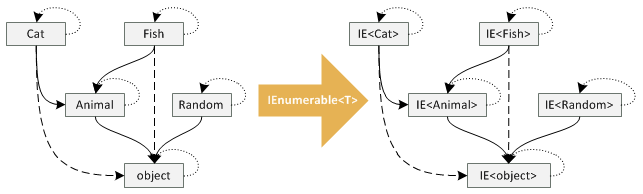
\includegraphics[width=0.7\textwidth]{covariantFunctors.png}

    \vspace{4mm}
    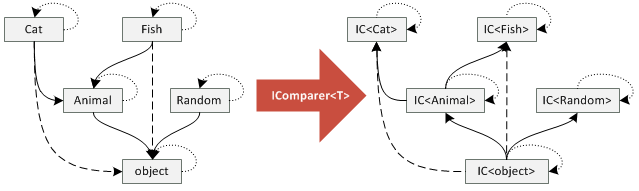
\includegraphics[width=0.7\textwidth]{contravariantFunctors.png}
\end{center}

\end{document}
